\chapter{Unikernel frameworks}
\label{chap:unikernels}

Σε αυτό το κεφάλαιο θα γίνει μία εισαγωγή στην έννοια των unikernels και το
σκοπό τους, ενώ θα παρουσιαστούν ορισμένα unikernel frameworks, τα οποία
μελετήθηκαν κατά τη διάρκεια αυτής της εργασίας. 

Ένας τυπικός ορισμός των unikernels αναφέρεται στη σελίδα
\href{http://unikernel.org/}{unikernel.org} και είναι ο εξής: 
\vspace{1ex}
\\
\textit{Τα Unikernels είναι εξειδικευμένες εικόνες μηχανής, με ένα
μοναδικό χώρο διευθύνσεων, τα οποία κατασκευάζονται χρησιμοποιώντας library
operating systems} \\
\vspace{1ex}

Αναλύοντας τον παραπάνω ορισμό μπορούμε εύκολα να συμπεράνουμε τα βασικά
χαρακτηριστικά των unikernels:
\begin{itemize}
	\item εξειδικευμένες εικονικές μηχανές: κάθε unikernel μπορεί να είναι
	διαφορετικός από τους υπόλοιπους. Κάθε ένας αφορά μία συγκεκριμένη
		εφαρμογή και φτιάχνεται γύρω από αυτήν.
	\item ένας μοναδικός χώρος διευθύνσεων: στην περίπτωση των unikernels
		δεν υπάρχει ο διαχωρισμός μεταξύ userspace και kernelspace, όπως
		στα συμβατικά λειτουργικά συστήματα.
	\item library operating systems ~\cite{porter2011rethinking}: πρόκειται
		για λειτουργικά συστήματα τα οποία παρέχουν τις υπηρεσίες που
		υποστηρίζουν (networking κ.λ.π.) στη μορφή βιβλιοθηκών, οι
		οποίες στη συνέχεια μπορούν να χρησιμοποιηθούν (link) από τις
		εφαρμογές. 
\end{itemize}

\begin{figure}[htp]
\centering
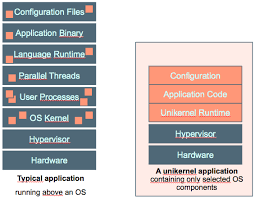
\includegraphics[scale=1]{figures/unikernel_vs_os.png}
\caption{Unikerne vs OS software stack\label{fig3_1}}
\end{figure}

Με λίγα λόγια ένας unikernel αποτελείται από τον κώδικα της εφαρμογής την οποία
θα εκτελέσει, τα απαραίτητα κομμάτια του λειτουργικού συστήματος που η
συγκεκριμένη εφαρμογή χρειάζεται και τις κατάλληλες παραμετροποιήσεις. Τα
unikernels δεδομένου ότι αφορούν μία και μόνο εφαρμογή δεν υποστηρίζουν
περισσότερες από μία διεργασίες, ούτε περισσότερους από έναν χρήστες. Αυτόματα
όλο το κομμάτι των συμβατικών λειτουργικών συστημάτων που αφορούν τη διαχείρηση
και υποστήριξη πολλών διεργασίων και χρηστών καθίσταται άχρηστο και δεν
συμπεριλαμβάνεται. Τα πράγματα είναι διαφορετικά όσον αφορά τα νήματα, καθώς
άλλα unikernel frameworks τα υποστηρίζουν ενώ άλλα όχι. 

Στην εικόνα ~\ref{fig3_1} φαίνεται η διαφορά μεταξύ ενός συμβατικού λειτουργικού
συστήματος και ενός unikernel. Τα παραπάνω ενοποιούνται σε μία εικόνα μηχανής
που μπορεί να εκτελεστεί από έναν επόπτη. Γίνεται εύκολα αντιληπτό ότι το
μέγεθος της τελικής εικόνας θα είναι πολύ μικρότερο από αυτή ενός συμβατικού
λειτουργικού συστήματος. Μία ακόμη συνέπεια αυτού είναι ότι οι χρόνοι εκκίνησης
θα είναι αρκετά μικρότεροι, αφού πλέον δε χρειάζεται να φορτωθούν και να
εκκινήσουν όλες οι υπηρεσίες που προσφέρει ένα λειτουργικό σύστημα. 

Από άποψη ασφάλειας, ο σχεδιασμός των unikernels από μόνος του προσφέρει
σημαντική ασφάλεια. Αρχικά το μικρό μέγεθος των unikernels συνεπάγεται αυτόματα
και μικρότερο εύρος επίθεσης από κάποιον κακόβουλο χρήστη. Επιπλέον πρόκειται
για εξειδικευμένες εικόνες που αφορούν μία και μόνο εφαρμογή, οπότε στην
περίπτωση που αποκτηθεί πρόσβαση στην εικονική μηχανή, το περιθώριο
εκμετάλλευσης θα είναι αρκετά μικρό. Τέλος, υπάρχει απομόνωση μεταξύ των
εικονικών μηχανών η οποία προσφέρεται από τον επόπτη. 

H έλλειψη διαχωρισμού kernelspace και userspace, μειώνει το κόστος
μετάβασης από τον ένα χώρο διευθύνσεων στον άλλο, κάνοντας έτσι τις κλήσεις
συστήματος να λειτουργούν σαν απλές κλήσεις συναρτήσεων. Ως αποτέλεσμα, η
ταχύτητα εκτέλεσης αυξάνει σημαντικά, καθώς δε χρειάζονται πλέον οι μεταβάσεις
από τον ένα χώρο διευθύνσεων στον άλλο, μία αρκετά δαπανηρή λειτουργία.
%% Από την άλλη τίθεται το ζήτημα της ασφάλειας 
%% grapse kati egia auto...

Η έννοια των library operating systems δεν είναι καινούρια, ωστόσο δεν μπορούσαν
να χρησιμοποιηθούν λόγω του μεγάλου πλήθους των συσκευών και συνεπώς των drivers
που θα έπρεπε να υποστηρίζουν. Στις μέρες μας όμως, οι επόπτες έχουν περιορίσει
σημαντικά το πλήθος των συσκευών κάνοντας εφικτή τη χρήση των συγκεκριμένων
λειτουργικών συστημάτων. 
 
Αφ' ετέρου η απομάκρυνση όλων αυτών των υπηρεσιών από το λειτουργικό σύστημα,
δημιουργεί αρκετούς περιορισμούς. Οι περισσότερες εφαρμογές έχουν φτιαχτεί για
συμβατικά λειτυργικά συστήματα λαμβάνοντας υπόψιν και χρησιμοποιοώντας τις
συγκεκριμένες υπηρεσίες. Απαιτείται, λοιπόν, να γίνουν σημαντικές αλλαγές στις
εφαρμογές για να μπορέσουν να εκτελεστούν σε unikernels. Επιπλέον γίνεται πιο
δύσκολη η αποσφαλμάτωση των unikernels δεδομένου των λίγοστών υπηρεσιών που
προσφέρουν. 

\section{Rumprun}
Το rumprun είναι ένα unikernel framework, το οποίο έχει χτιστεί με βάση τα
συστατικά των drivers που προσφέρουν οι rump kernels. 
To rumprun μπορεί να προσφέρει ένα POSIX-like περιβάλλον, το οποίο μπορεί να
χρησιμοποιηθεί από POSIX εφαρμογές ώστε να μετατραπούν χωρίς καμία αλλαγή σε
unikernel εικόνες. Αυτός ήταν και ένας από τους βασικούς στόχους του
εγχειρήματος, η δυνατότητα δηλαδή σε POSIX κώδικα να μπορεί να εκτελεστεί χωρίς
να υποστεί καμία αλλαγή. Στην εικόνα \ref{fig3_2} φαίνεται η δομή του rumprun
για POSIX εφαρμογές (αριστερά) και προσαρμοσμένες εφαρμογές (δεξιά). Προφανώς το
δεξί μοντέλο φαίνεται αρκετά μικρότερο, αλλά είναι απαραίτητες να γίνουν
συγκεκριμένες αλλαγές στην εφαρμογή. O συγκεκριμένος unikernel μπορεί να
εκτελεστεί χρησιμοποιώντας Xen ή KVM, ενώ υποστηρίζει arm και x86
αρχιτεκτονικές. Ο κώδικας του rumprun είναι διαθέσιμος στο
\url{http://repo.rumpkernel.org/rumprun}. 

\begin{figure}[htp]
\centering
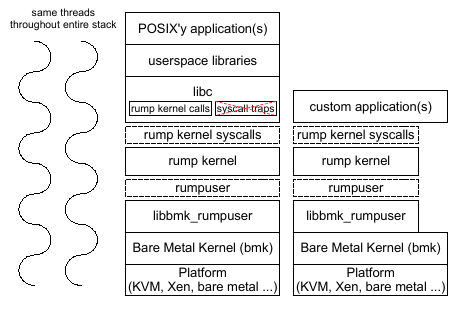
\includegraphics[scale=0.75]{figures/rumprun_stack.png}
\caption{Rumprun software stack\label{fig3_2}}
\end{figure}

Όπως κάθε unikernel framework το rumprun υποστηρίζει μία και μόνο διεργασία.
Μολαταύτα υποστηρίζει POSIX threads, δίνοντας τη δυνατότητα για την ύπαρξη
περισσοτέρων από ένα νήματα. Μάλιστα ο χρονοδρομολογητής που διαθέτει είναι
cooperative, οπότε αν ένα νήμα αποκτήσει τον έλεγχο δνε πρόκειται να διακοπεί
από το χρονδορομοληγτή αλλά θα αφήσει το έλεγχο όταν εκείνο τερματίσει ή
πρόκειται να μπλοκάρει. Κάποιοι ακόμα περιορισμοί, είναι η μη υποστήριξη
εικονικής μνήμης (virtual memory) και σημάτων (signals), Συνεπώς εφαρμογές που
χρησιμοποιούν σήματα ή κλήσεις συστήματος όπως η mmap() δε θα λειτουργούν χωρίς αλλαγές στον κώδικα τους.

Ένας rumprun unikernel αποτελείται από τα απαραίτητα κομμάτια των rump kernels
που χρειάζεται η εφαρμογή και την ίδια την εφαρμογή. Για τη δημιουργία του
unikernel γίνεται πάντα cross-compilation, οπότε δε χρειάζεται κάποιος ήδη
´ετοιμος rumprun unikernels, αλλά μία σειρά από εργαλεία. H διαδικασία έχει ως
εξής:
\begin{enumerate}
	\item Αρχικά γίνεται η μεταγλώττιση του κώδικα της εφαρμογής
		χρησιμοποιοώντας έναν cross-compiler.
	\item Ύστερα, αντί για linking γίνεται pseudo-linking όπως ονομάζουν τη
		διαδικασία κατά την οποία απλά ελέγχονται αν ικανοποιούνται όλες
		οι εξαρτήσεις συμβόλων, χωρίς να γίνεται κάποια σύνδεση με
		κάποιο συστατικό του λειτουργικού συστήματος.
	\item Τέλος, το παράγωγο του προηγούμενου βήματος γίνεται "bake", όπου
		εισάγονται και τα κομμάτια του λειτουργικού συστήματος που
		απαιτούνται, όπως έχουν οριστεί κατά την εκτέλεση της εντολής.
\end{enumerate}

Όπως έχει αναφερθεί ο rumprun unikernel βασίζεται στα rump kernels
~\cite{rumprun_Xen}. Τα rump kernels παρέχουν drivers του NetBSD ως φορητά
εξαρτήματα με τα οποία μπορείς να εκτελέσεις εφαρμογές χωρίς να ναι απαραίτητη η
ύπαρξη λειτουργικού συστήματος ~\cite{kantee2014rump}. Η αρχική ιδέα ήταν να
υπάρχει η δυνατότητα να εκτελούνται αμετάβλητοι drivers του NetBSD ως απλά
προγράμματα σε userspace, ώστε να είναι πιο εύκολος ο έλεγχος και η ανάπτυξη
NetBSD drivers. Ένας rump kernel είναι ένας πυρήνας χρονομερισμού (timesharing)
από τον οποίο έχουν αφαιρεθεί ορισμένα κομμάτια ~\cite{kantee2012design}. Τα
κομμάτια που κρατήθηκαν είναι οι drivers και οι απαραίτητες ρουτίνες που
χρειάζονται οι συγκεκριμένοι drivers για να λειτουργήσουν (συχχρονισμός,
κατανομή μνήμης κ.λ.π.). Τα κομμάτια που αφαιρέθηκαν είναι αυτά που αφορούν τις
διεργασίες, την εικονική μνήμη κ.α.. Επιπλέον τα rump kernels έχουν και ένα
καλώς ορισμένο στρώμα φορητότητας, ώστε να είναι εύκολο να ενσωματωθούν σε
διάφορα περιβάλλοντα.

Πίσω από τα rump kernels υπάρχει μία ακόμα έννοια αυτή του
anykernel ~\cite{kantee2012design}. O συγκεκριμένος όρος δημιουργήθηκε
ως απάντηση στην όλο και αυξανόμενο αριθμό μοντέλων λειτουργικών συστημάτων
(monolithic, exokernel, mikrokernel, unikernel κ.λ.π.). Ένα πολύ μεγάλο ποσοστό
ενός λειτουργικού συστήματος ανεξάρτητα από το μοντέλο που χρησιμοποιεί
αποτελείται από drivers. Ο όρος anykernel περιγράφει ένα κώδικα βάσης (codebase)
τύπου κώδικα πυρήνα από τον οποίο οι οδηγοί μπορούν να εξαχθούν και να
ενσωματωθούν σε οποιοδήποτε μοντέλο λειτουργικού συστήματος, χωρίς να
χρειάζονται αλλαγές και συντήρηση. Στην εικόνα ~\ref{fig3_3} φαίνεται η σχέση
μεταξύ των εννοιών anykernel, rump kernels και rumprun. 


\begin{figure}[htp]
\centering
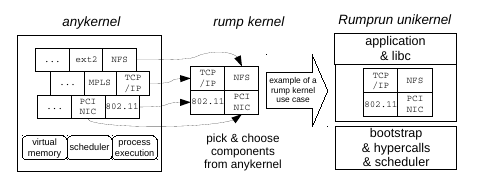
\includegraphics[scale=0.8]{figures/from_anykernel_to_rump.png}
\caption{Σχέση μεταξύ των ενοιών anykernel, rump kernel και rumprun\label{fig3_3}}
\end{figure}

\section{OSv}
Το OSv δημιουργήθηκε από το μηδέν, με σκοπό να μπορεί να εκτελέσει μία εφαρμογή
πάνω από έναν επόπτη. Ως γλώσσα προγραμματισμού χρησιμοποιεί τη C++ και ο
κώδικας του είναι διαθέσιμος στο \url{https://github.com/cloudius-systems/osv}. 
Υποστηρίζει διάφορους επόπτες και επεξεργαστές, όπως arm και x86, ενώ στην
x86 αρχιτεκτονική υποστηρίζει τους επόπτες Xen, KVM, VMWare, Virtualbox. Παρέχει
τη δυνατότητα να μπορεί να υποστηρίξει σχεδόν οποιοδήποτε πρόγραμμα, που δε
χρειάζεται παραπάνω από μία διεργασία. Μάλιστα παρέχει υποστήριξη για αρκετές
γλώσσες προγραμματισμού όπως C, Java, Ruby, Node.js, Perl και άλλες. 

\begin{figure}[htp]
\centering
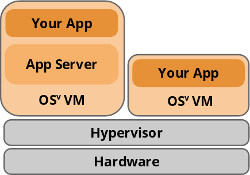
\includegraphics[scale=0.8]{figures/osv.jpg}
\caption{Osv unikernel stack\label{fig3_4}}
\end{figure}

Η επιλογή των δημιουργών του OSv να δημιουργήσουν από την αρχή ένα νέο
λειτουργικό σύστημα τους έδωσε τη δυνατότητα να εισάγουν ορισμένες νέες
τεχνικέaς ~\cite{kivity2014v}. Σε αυτό το πλαίσιο στο OSv δεν υπάρχουν
spinlocks. Στα περισσότερα SMP (Symmetric multiprocessing)
λειτουργικά συστήματα χρησιμοποιούνται spinlocks για την προστασία κοινών
δεδομένων από πολλά νήματα. Όταν ένα νήμα κατέχει το spinlock για μία δομή
δεδομένων τα υπόλοιπα νήματα δεν μπορούν να αποκτήσουν πρόσβαση στη συγκεκριμένη
δομή και περιμένουν, κάνοντας συνεχώς ερωτήματα αν το κλείδωμα είναι ελεύθερο.
Τα spinlocks χρησιμοποιούνται κυρίως για νήματα που δεν μπορούν να μπλοκάρουν
(κυρίως νήματα του πυρήνα). Ωστόσο, στην περίπτωση της εικονικοποίησης τα
spinlocks δημιουργούν το πρόβλημα του "lock-holder preemption”
~\cite{uhlig2004towards}. Αν μία εικονική CPU σταματήσει να εκτελείται και
κρατάει ένα spinlock, οι άλλες CPU που χρειάζονται το συγκεκριμένο spinlock,
είναι αναγκασμένες να περιμένουν σπαταλώντας κύκλους της CPU. Υπό αυτές τις
συνθήκες στο OSv αποφάσισαν όλη η δουλειά του πυρήνα να γίνεται από νήματα που
μπορούν να "κοιμηθούν". Τα παραπάνω δεν ισχύουν για το χρονοδρομολογητή, ο
οποίος δεν μπορεί να "κοιμηθεί", οπότε χρησιμοποιεί ουρές εκτέλεσης για κάθε
επεξεργαστή, ωστε να μην απαιτείται συννενόηση μεταξύ των επεξεργαστών για τη
χρονοδρομολόγηση, ενώ αν ένα νήμα αλλάξει επεξεργαστή χρησιμοποιούνται lock-free
αλγόριθμοι.

Όπως αναφέρθηκε προηγουμένως το OSv διαθέτει χρονδορομολογητή. Μερικά από τα
χαρακτηριστικά του είναι: διακοπτόμενη χρονδορομολόγηση (preemptive scheduling),
η μη χρήση spinlocks και χωρίς timer interrupts, ενώ τέλος δε γίνεται κανένας
διαχωρισμός μεταξύ των νημάτων του πυρήνα και της εφαρμογής. Ένα εξίσου
ενδιαφέρον κομμάτι στο σχεδιασμό του OSv είναι το network stack. Λαμβάνοντας
υπόψιν ότι πρόκειται για ένα λειτουργικό συστημα για το cloud, το OSv έχει δώσει
μεγάλη βαρύτητα στην υποστήριξη εφαρμογών που χρησιμοποιούν πολύ το δίκτυο. Το
network stack λοιπόν, είναι σχεδιασμένο με βάση τις ιδέες του Van Jacobson
~\cite{jacobson2006speeding}, με βάση τις οποίες το OSv υποστηρίζει ότι
πετυχαίνει πολύ υψηλότερη απόδοση από τα network stacks των συμβατικών
λειτουργικών συστημάτων. 

H εκτέλεση μίας εφαρμογής στο OSv δε διαφέρει αρκετά από την εκτέλεση της σε ένα
συμβατικό λειτουργικό σύστημα, όπως π.χ. το Linux. Η διαφορά είναι ότι στο OSv
δεν εκτελούνται τα συνηθισμένα fixed-position εκτελέσιμα αλλά απαιτούνται shared
objects. Για την εκτέλεση του το OSv αναζητά την main συνάρτηση της εφαρμογής
και την εκτελεί. Για το πως θα τοποθετηθεί η εφαρμογή στο unikernel,
προσφέρονται δύο τρόποι. Εϊτε όταν χτίζεται το unikernel ορίζουμε να
συμπεριληφθεί και το αντίστοιχο shred object, είτε μπρορούμε να το φορτώσουμε
στο unikernel μεταγενέστερα, μέσω του REST API που προσφέρει το OSv. Μάλιστα,
υπάρχει η επιλογή για διαχείρηση του unikernel μέσω μία ιστοσελίδας, ενώ υπάρχει
η δυνατότητα να υπάρχει ένα απλό κέλυφος (shell). Αξιοσημείωτη είναι και η
προσπάθεια δημιουργίας ενός εργαλείου για τη δημιουργία unikernels με OSv. Το
εργαλείο αυτό ονομάζεται Capstan και μοιάζει αρκετά στη χρήση του με το Docker.

Σαν γενική εικόνα το OSv μοιάζει με ένα library operating system, το οποίο
υποστηρίζει πολλές λειτουργίες των συμβατικών λειτυργικών συστημάτων. Ενδεικτικό
είναι το γεγονός ότι διαθέτει εικονική μνήμη, καθώς και ένα εικονικό σύστημα
αρχείων. Χάρις όλα αυατά τα χαρακτηριστικά μπορεί να υποστηρίξει ένα πολύ μεγάλο
εύρος εφαρμογών ακόμα και αυτές που κάνουν χρήση της mmap(). Ο μόνος περιορισμός
που υπάρχει είναι ότι δεν υποστήριζεται η fork(), καθώς παραβιάζει το
single-process χαρακτήρα. Από την άλλη μεριά, όλες αυτές οι λειτουργίες που
προσφέρονται αυξάνουν το μέγεθος του unikernel, κάνοντας το OSv ένα από τα πιο
"βαριά" unikernel frameworks. 


\section{Linux Kernel Library - lkl}
To lkl ~\cite{purdila2010lkl} φέρνει τις ιδέες του rumpkernel και του anykernel
στο Linux. Βασικός στόχος του είναι η επαναχρησιμοποίηση του κώδικα του Linux με
όσο το δυνατόν λιγότερη προσπάθεια και μειωμένο κόστος συντήρησης. Έχει
υλοποιηθεί ως ένα port του Linux σε μία εικονική αρχιτεκτονική (lkl),
προκειμένου να μειωθούν οι ενοχλητικές τροποποιήσεις του πυρήνα. Το lkl μπορεί
να χρησιμποιηθεί για τρεις διαφορετικούς λόγους, α) στιγμιαία παράκαμψη του
πυρήνα, β) επαναχρησιμοποίηση κώδικα πυρήνα στο χώρο χρήστη και τέλος γ) ως
unikernel. Βασικά χρησιμοποιείται περισσότερο για τη χρήση ορισμένων
λειτουργειών του πυρήνα του Linux σε άλλα λειτουργικά σσυτήματα ή στο χώρο
χρήστη, παρά ως unikernel.

Το lkl στην ουσία είναι βιβλιοθήκες τις οποίες οι εφαρμογές μπορούν να
χρησιμοποιήσουν. Για τη χρήση του, λοιπόν, προσφέρει ένα δικό του ΑΡΙ, που
αποτελεί ένα υποσύνολο των κλήσεων συστήματος του Linux. Στην εικόνα
~\ref{fig3_6} φαίνονται όλα τα συστατικά του lkl. Όπως φαίνεται υπάρχουν δύο
APIs 1) lkl system call API, που είναι βασισμένο στις κλήσεις συστήματος του
Linux  και 2) το API που χρησιμοποιεί το πρώτο έμμεσα. Το δεύτερο API
αποτελείται από τη hijack library και μία βασική υλοποίηση βιβιλιοθήκης και
συγκεκριμένα μία τροποποίηση της musl libc ώστε να χρησιμοποιεί το lkl system
call API. H hijack library χρησιμοποιείται για την επί τόπου αντικατάσταση των
κλήσεων συστήματος που εκτελεί μία εφαρμογή, ώστε να μπορεί η εφαρμογή να
χρησιμοποιεί το lkl αντί για τον πυρήνα του host. 

\begin{figure}[htp]
\centering
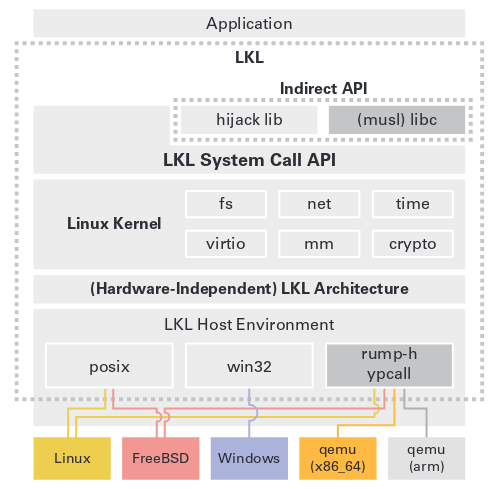
\includegraphics[scale=0.6]{figures/lkl.png}
	\caption{Η αρχιτεκτονική του lkl\label{fig3_6}}
\end{figure}

Τα υπόλοιπα κομμάτια του lkl έχουν να κάνουν με το περιβάλλον του host και την
generic lkl architecture. Δεδομένου, ότι το lkl δε στοχεύει μόνο σε ένα
περιβάλλον, δε χρησιμοποιεί κώδικα που εξαρτάται από την πλατφόρμα. Αντ' αυτού η
εφαρμογή θα πρέπει να υλοποιεί ορισμένα θεμελιακά στοιχεία που εξαρτόνται από το
περιβάλλον. Αυτά τα θεμελιακά στοιχεία χρησιμοποιούνται από την lkl generic
architecture για τη δημιουργία της εικονικής μηχανής πάνω στην οποία θα
εκετελεστεί ο πυρήνας του Linux. Ωστόσο, υπάρχουν ορισμένα περιβάλλοντα για τα
οποία το lkl παρέχει αυτά τα θεμελιακά στοιχεία. Τα περιβάλλοντα αυτά είναι το 
POSIX, το ΝΤ (windows userspace), το NTK (Windows kernel), το Apache Portable
Runtime, ενώ υπάρχει υποστήριξη και για το rumprun. 

Το lkl επιτρέπει την εκτέλεση μίας και μόνο διεργασίας, ενώ παρέχει υποστήριξη
για πολλαπλά νήματα με ορισμένους περιορισμούς. Αρχικά δεν υπάρχει υποστήριξη
για SMP και επιπλέον μία εφαρμογή περιορίζεται απλά στη δημιουργία και τον
τερματισμό ένός νήματος. Όσον αφορά τη διαχείρηση της μνήμης, αφού δε χρειάζεται
κάποια προστασία μνήμης το lkl απλά χρειάζεται ένα χώρο μνήμης από τον οποίο
μπορεί ο πυρήνας του Linux να κατανείμει μνήμη που χρειάζεται. Επιπλέον χάρις τη
δυνατότητα του Linux να παρέχει εικονική μνήμη ακόμα και για non-MMU
αρχιτεκτονικές μπορεί να υποστηριχθεί και εικονική μνήμη. 
%% isws na anaferw kai ti prosferei (no smp, multi threadsed)

\section{IncludeOS}
To IncludeOS ~\cite{bratterud2015includeos} είναι ένα από τα νεώτερα Unikernel
frameworks. Είναι γραμμένο σε C++ και υποστηρίζει εφρμογές που χρησιμοποιούν την
ίδια γλώσσα προγραμματισμού. Βασικός στόχος για το συγκεκριμένο unikernel είναι
να έχει τόσο απλή χρήση όσο η χρήση μίας βιβλιοθήκης στη C++. Πιο συγκεκριμένα
μία εντολή της μορφής \#include <os> στην αρχή μίας εφαρμογής θα έχει ως
αποτέλεσμα το χτίσιμο μίας εικόνας δίσκου (disk image) που μπορεί να εκετελεστεί
από τους περισσότερους επόπτες (kvm, virtualbox). Για να υπάρχει αυτή η
δυνατότητα οι δημιουργοί του IncludeOS, έχουν αναπτύξει και μία σειρά εργαλείων.
Χρησιμοποιώντας τα, η διαδικασία του "χτισίματος" περιλαμβάνει τρία στάδια.
Αρχικά, γίνεται η σύνδεση της εφαρμογής με τα μέρη του λειτουργικού συστήματος
που χρειάζονται. Στη συνέχεια, προσάπτεται o boot loader και τέλος όλα αυτά
ενοποιούνται σε ένα disk image. Η διαδικασία του χτισίματος φαίνεται και στην
εικόνα ~\ref{fig3_5}. 

\begin{figure}[htp]
\centering
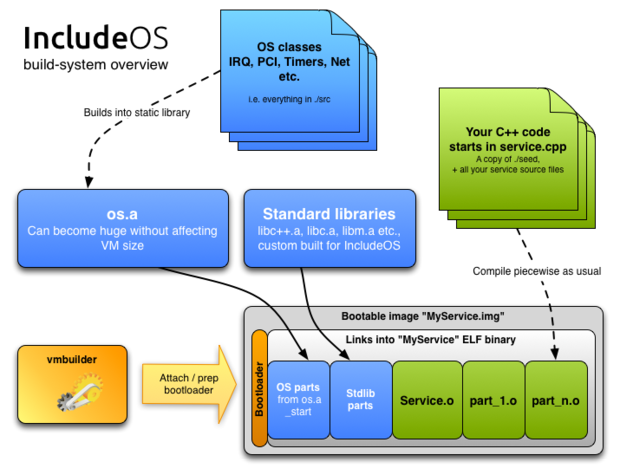
\includegraphics[scale=0.6]{figures/includeos_buil_system.png}
\caption{IncludeOS building process\label{fig3_5}}
\end{figure}

Αρκετά ενδιαφέρουσες είναι και ορισμένες σχεδιαστικές επιλογές των δημιουργών
που αφορούν κυρίως το network stack. Χρησιμοποιεί έναν virtio driver για την
επικοινωννία με τον επόπτη, συνεπώς δε χρειάζεται ο τελευταίος να προσομοιώνει
διάφορες συσκευές αλλά απλά να χρησιμοποιεί το virtio. Επιπροσθέτως, η επιλογή
να φτιαχτεί από την αρχή το συγκεκριμένο framework, έδωσε τη δυνατότητα στη
δημιουργία ενός νέου TCP-IP stack, χρησιμοποιώντας σε μεγάλο βαθμό τις
δυνατόττητες που έδινε η C++. Τέλος, τo IncludeOS δεν έχει κάποιο τρόπο να
φορτώσει ένα πρόγραμμα, συνεπώς δεν υπάρχει η κλασσική main συνάρτηση. Αντ'
αυτού, υπάρχει η κλάση Service και ο προγραμματιστής πρέπει να υλοποιήσει την
Service::start η οποία θα κληθεί μετά την αρχικοποίηση του λειτουργικού
συστήματος. 

Όπως έχει αναφερθεί προηγουμένως, μόνο C++ προγράμματα μπορούν να εκτελεστούν
στο IncludeOS, ενώ μπορεί να χρησιμοποιηθεί και η standard βιβλιοθήκη της C. Με
αυτό τον τρόπο υπάρχει μία μερική υποστήριξη για POSIX εφαρμογές. Ιδιαίτερα
λειτουργίες που αφορούν την είσοδο/έξοδο (Ι/Ο) και τα νήματα δεν υποστηρίζονται.
Στο IncludeOS όλη η εργασία γίνεται από ένα και μόνο νήμα, χωρίς I/O μπλοκάρισμα
ή context switching μέσα στο guest, με το συγκεκρμένο μοντέλο να θυμίζει εκείνο
του Node.js. Όπως και στα υπόλοιπα unikernel frameworks μόνο μία διεργασία
μπορεί να υπάρχει ανά unikernel, ενώ δεν υπάρχει και εικονική μνήμη.


\section{ClickOS}
Τα frameworks που έχουν παρουσιαστεί μέχρι στιγμής υποστηρίζουν ένα ευρύ φάσμα
εφαρμογών. To ClickOS αντιθέτως έχει συγκεκριμένο στόχο, τις εφαρμογές που
υλοποιούν διάφορες λειτουργίες δικτύου. 

%%NFV
%%TinyOS

\section{Mirage OS}
dsfdsgfdsgdfs


